\section{Cursograma Producci\'on}
\begin{center}
 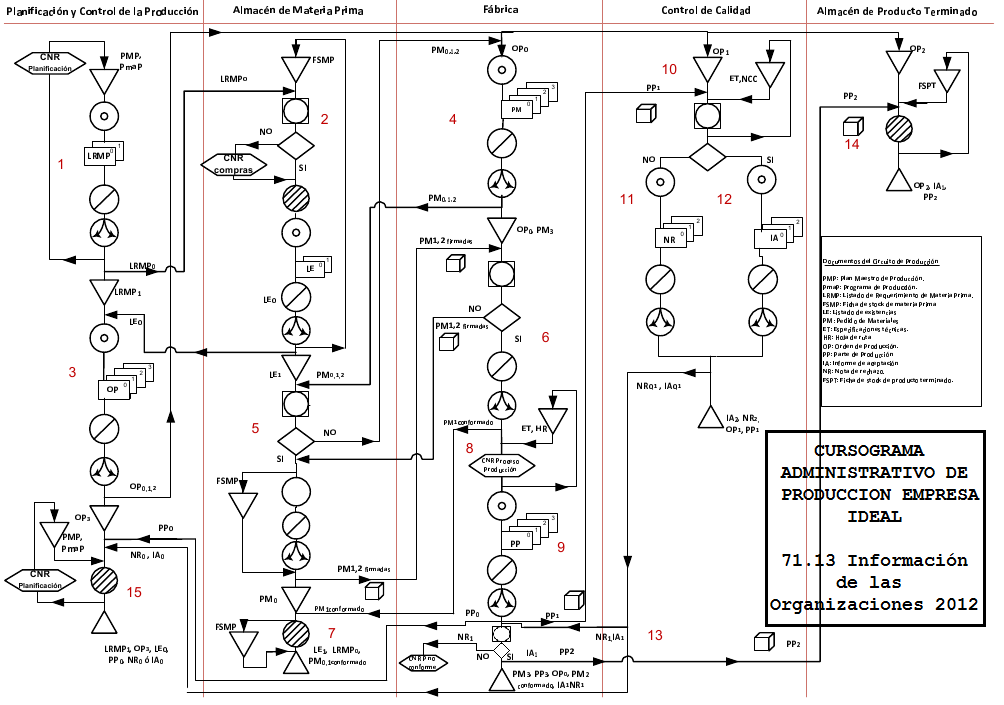
\includegraphics[angle=90,scale=0.95,keepaspectratio=true]{./Circuitos-Teoricos/Produccion/Images/cursograma-produccion.png}
 % cursograma-produccion.png: 1004x705 pixel, 96dpi, 26.56x18.65 cm, bb=0 0 753 529
\end{center}

\section{Procedimiento de Producci\'on}
\begin{center}
 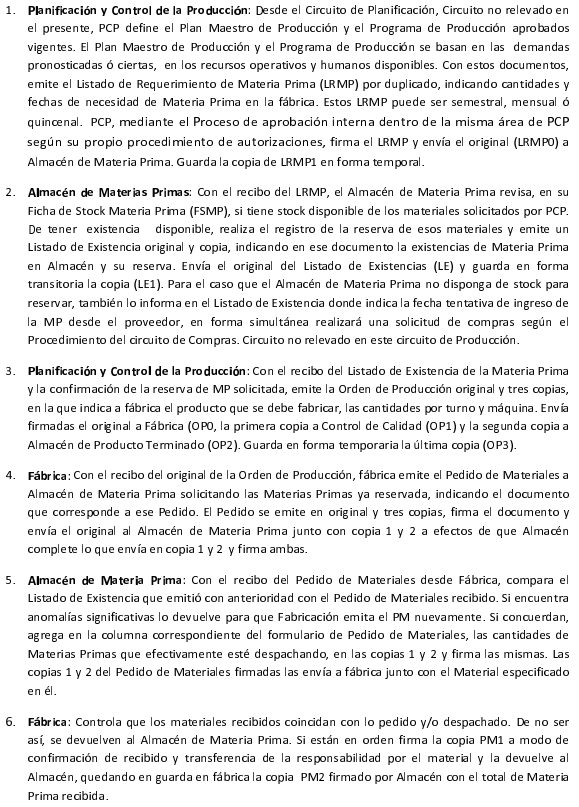
\includegraphics[keepaspectratio=true]{./Circuitos-Teoricos/Produccion/Images/procedimiento-produccion.png}
 % procedimiento-produccion.png: 579x807 pixel, 96dpi, 15.32x21.35 cm, bb=0 0 434 605
\end{center}
\begin{center}
 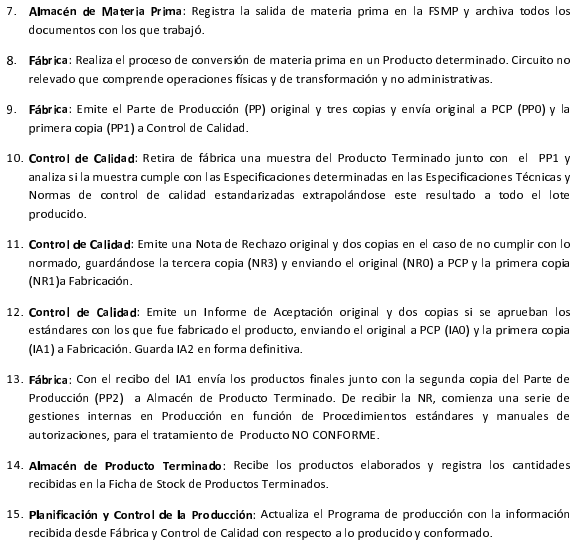
\includegraphics{./Circuitos-Teoricos/Produccion/Images/procedimiento-produccion-2.png}
 % procedimiento-produccion-2.png: 576x545 pixel, 96dpi, 15.24x14.42 cm, bb=0 0 432 409
\end{center}

\pagebreak
\section{Cursograma de Producci\'on (con numeración para el manual)}
\subsection{Manual del Cursograma de Producci\'on}

\begin{center}\textbf{Sectores intervinientes}\end{center}
\begin{itemize}
  \item Planificaci\'on y Control de Producci\'on.
  \item Almac\'en de Materia Prima.
  \item F\'abrica.
  \item Control de Calidad.
  \item Almac\'en de Producto Terminado.
\end{itemize}

\begin{center}
  \textbf{Documentos}
  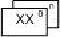
\includegraphics{./Images/Simbolos/simbolo-Documentos.png}
\end{center}
\begin{enumerate}
  \item Listado de Requerimientos de Materia Prima (LRMP).
  \item Orden de Producci\'on (OP).
  \item Listado de Existencia (LE).
  \item Pedido de Materiales (PM).
  \item Parte de Producci\'on (PP).
  \item Nota de Rechazo (NR).
  \item Informe de Aceptaci\'on (IA).
  \item Ficha de Stock de Materia Prima (FSMP).
  \item Ficha de Stock de Producto Terminado (FSPT).
  \item Plan Maestro de Producci\'on (PMP).
  \item Programa de Producci\'on (PmaP).
  \item Especificaciones t\'ecnicas (ET).
  \item Hoja de Ruta (HR).
  \item Normas de Control de Calidad (NCC).
\end{enumerate}

\begin{center}
  \textbf{Emisión de Documentos}
  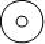
\includegraphics{./Images/Simbolos/simbolo-Emision-de-Documentos.png}
\end{center}
\begin{enumerate}
  \item Planificaci\'on y Control de la Producci\'on: emite el LRMP, original y copia.
  \item Planificaci\'on y Control de la Producci\'on: emite la OP, original y tres copias. 
  \item Almac\'en de Materia Prima: emite un LE, original y copia.
  \item F\'abrica: emite el PM, original y tres copias.
  \item F\'abrica: emite el PP, original y tres copias.
  \item Control de Calidad: emite una NR, original y dos copias.
  \item Control de Calidad: emite un IA, original y dos copias.
\end{enumerate}

\begin{center}
  \textbf{Firma}
  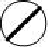
\includegraphics{./Images/Simbolos/simbolo-Firma.png}
\end{center}
\begin{enumerate}
  \item Planificaci\'on y Control de la Producci\'on: se firman las LRMP.
  \item Planificaci\'on y Control de la Producci\'on: se firman las OP.
  \item Almac\'en de Materia Prima: se firman las LE.
  \item Almac\'en de Materia Prima: se firman PM primera y segunda copia.
  \item F\'abrica: se firman los PM.
  \item F\'abrica: se firma la PM primera copia conformada.
  \item F\'abrica: se firman PP.
  \item Control de Calidad: se firman las NR.
  \item Control de Calidad: se firman los IA.
\end{enumerate}

\begin{center}
  \textbf{Distribución}
  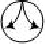
\includegraphics{./Images/Simbolos/simbolo-Distribucion.png}
\end{center}
\begin{enumerate}
  \item Planificaci\'on y Control de la Producci\'on: distribuye LRMP original a Almac\'en de Materia Prima; y converva la copia.
  \item Planificaci\'on y Control de la Producci\'on: distribuye OP original a F\'abrica, la primera copia a Control de Calidad y la segunda copia a Almac\'en de Producto Terminado; conserva la \'ultima copia.
  \item Almac\'en de Materia Prima: distribuye LE original a Planificaci\'on y Control de la Producci\'on; conserva la copia.
  \item Almac\'en de Materia Prima: distribuye PM primera y segunda copia a F\'abrica; conserva el original. \item F\'abrica: distribuye PM original y las dos primeras copias a Almac\'en de Materias Primas; conserva la \'ultima copia.
  \item F\'abrica: distribuye PM primera copia a Almac\'en de Materias Primas. 	
  \item F\'abrica: distribuye PP original a Planificaci\'on y Control de la Producci\'on, la primera copia a Control de Calidad, y la segunda copia a Almac\'en de Producto Terminado; conserva la \'ultima copia.
  \item Control de Calidad: distribuye NR original a Planificaci\'on y Control de la Producci\'on y la primera copia a F\'abrica; conserva la segunda copia.
  \item Control de Calidad: distribuye IA original a Planificaci\'on y Control de la Producci\'on y la primera copia a F\'abrica; conserva la segunda copia.
\end{enumerate}

\begin{center}
  \textbf{Almacenamiento Transitorio}
  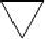
\includegraphics{./Images/Simbolos/simbolo-Almacenamiento-Transitorio.png}
\end{center}
\begin{enumerate}
  \item Planificaci\'on y Control de la Producci\'on: almacena de manera transitoria PMP y PmaP.
  \item Planificaci\'on y Control de la Producci\'on: almacena de manera transitoria LRMP copia.
  \item Planificaci\'on y Control de la Producci\'on: almacena de manera transitoria OP tercera copia.
  \item Planificaci\'on y Control de la Producci\'on: almacena de manera transitoria PMP y PmaP.
  \item Almac\'en de Materia Prima: almacena de manera transitoria FSMP.
  \item Almac\'en de Materia Prima: almacena de manera transitoria LE copia.
  \item Almac\'en de Materia Prima: almacena de manera transitoria FSMP.
  \item Almac\'en de Materia Prima: almacena de manera transitoria PM original.  
  \item Almac\'en de Materia Prima: almacena de manera transitoria FSMP.
  \item F\'abrica: almacena de manera transitoria OP original y PM tercera copia.
  \item F\'abrica: almacena de manera transitoria ET y HR.
  \item Control de Calidad: almacena de manera transitoria OP primera copia.
  \item Control de Calidad: almacena de manera transitoria ET y NCC.
  \item Almac\'en de Producto Terminado: almacena de manera transitoria OP segunda copia.
  \item Almac\'en de Producto Terminado: almacena de manera transitoria FSPT.
\end{enumerate}

\begin{center}
  \textbf{Control y verificación}
  
\includegraphics{./Images/Simbolos/simbolo-Control-y-Verificacion.png}
\end{center}
\begin{enumerate}
  \item Almac\'en de Materia Prima: controla y verifica si tiene stock disponible de los materiales solicitados por Planificaci\'on y Control de la Producci\'on, comparando LRMP recibido y FSMP.
  \item Almac\'en de Materia Prima: controla y verifica si concuerda el pedido de materiales, comparando PM recibido de F\'abrica y el LE emitido anteriormente.
  \item F\'abrica: controla y verifica si los materiales recibidos coincidan con lo pedido y/o despachado.
  \item Control de Calidad: controla y verifica si la muestra del Producto Terminado recibida cumple con las especificaciones determinadas en las ET,
\end{enumerate}

\begin{center}
  \textbf{Decisión}
  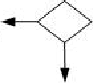
\includegraphics{./Images/Simbolos/simbolo-Decision.png}
\end{center}
\begin{enumerate}
  \item Almac\'en de Materia Prima: Si se tiene el stock disponible se registra la reserva de los materiales y se emite LE; caso contrario se emite LE con una fecha tentativa de ingreso de materia prima desde el proveedor, en forma simult\'anea se realiza una solicitud de compra seg\'un el Procedimiento del circuito de Compras (CNR).
  \item Almac\'en de Materia Prima: Si el PM es correcto entonces se procede a enviar el material; caso contrario lo devuelve a F\'abrica para que emita el PM nuevamente.
  \item F\'abrica: Si los materiales recibidos son los correctos se contin\'ua con la descarga; caso contrario se devuelven los materiales al Almac\'en de Materia Prima.
  \item F\'abrica: Si se recibe el AI se procede al env\'io de los materiales al Almac\'en de Producto Terminado. Si se recibe el NR, se comienza una serie de gestiones internas en funci\'on de Procedimientos est\'andares y manuales de autorizaciones, para el tratamiento de Producto NO CONFORME.
  \item Control de Calidad: Si la muestra pasa los controles de calidad, entonces se procede a emitir el IA; caso contrario se emite una NR.
\end{enumerate}

\begin{center}
  \textbf{Operación}
  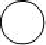
\includegraphics{./Images/Simbolos/simbolo-Operacion.png}
\end{center}
\begin{enumerate}
  \item Almac\'en de Materia Prima: Agrega en la columna correspondiente del formulario PM, la cantidad de materia prima que efectivamente se est\'e despachando.
\end{enumerate}

\begin{center}
  \textbf{Registro}
  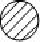
\includegraphics{./Images/Simbolos/simbolo-Registro.png}
\end{center}
\begin{enumerate}
  \item Planificaci\'on y Control de la Producci\'on: registra
  \item Almac\'en de Materia Prima: registra la reserva de materias primas en el LE.
  \item Almac\'en de Materia Prima: registra la salida de materia prima en la FSMP.
  \item Almac\'en de Producto Terminado: registra las cantidades recibidas de productos elaborados en la FSPT.
\end{enumerate}

\begin{center}
  \textbf{Almacenamiento definitivo}
  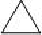
\includegraphics{./Images/Simbolos/simbolo-Almacenamiento-Definitivo.png}
\end{center}
\begin{enumerate}
  \item Planificaci\'on y Control de la Producci\'on: almacena de manera definitiva LRMP copia, OP tercera copia, LE original, PP original y NR original o IA original seg\'un corresponda.
  \item Almac\'en de Materia Prima: almacena de manera definitiva LE copia, LRMP original, PM original y primera copia conformada. 
  \item F\'abrica: almacena de manera definitiva PM tercera copia, PP tercera copia, OP original, PM segunda copia conformada y NR copia o IA copia seg\'un corresponda.
  \item Control de Calidad: almacena de manera definitiva OP primera copia, PP primera copia y IA segunda copia o NR segunda copia seg\'un corresponda.
  \item Almac\'en de Producto Terminado: almacena de manera definitiva OP segunda copia, IA primera copia y PP segunda copia.
\end{enumerate}

\begin{center}
  \textbf{Circuito no relevado}
  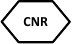
\includegraphics{./Images/Simbolos/simbolo-CNR.png}
  % simbolo-CNR.png: 73x44 pixel, 96dpi, 1.93x1.16 cm, bb=0 0 55 33
\end{center}
\begin{enumerate}
  \item Planificaci\'on y Control de la Producci\'on: Planificaci\'on.
  \item Almac\'en de Materia Prima: Compras.
  \item F\'abrica: Proceso Producci\'on.\
  \item F\'abrica: Tratamiento de Producto NO CONFORME.
\end{enumerate}

\pagebreak
\section{Formularios de Producci\'on}

\subsection{Orden de Producci\'on}
\begin{center}
 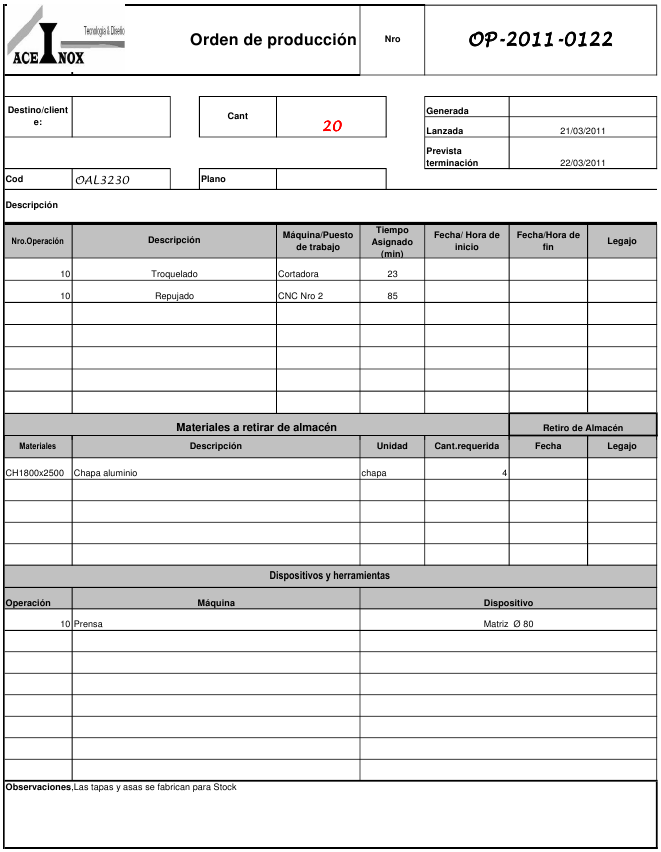
\includegraphics[scale=0.9,keepaspectratio=true]{./Circuitos-Teoricos/Produccion/Images/orden-de-produccion.png}
 % orden-de-produccion.png: 661x852 pixel, 96dpi, 17.49x22.54 cm, bb=0 0 496 639
\end{center}

\pagebreak
\begin{itemize}
 \item \textbf{Objetivo}: Es un documento en el que se especifican las operaciones que deben realizar la producci\'on.
 \item \textbf{Alcance}: Es un documento interno de la empresa.
\end{itemize}

\subsubsection{Descripción}
\begin{enumerate}
 \item Logo de la empresa.
 \item Número de Orden de Producci\'on.
 \item Cliente / Destino.
 \item Cantidad a realizar.
 \item Fecha de generaci\'on de la Orden de Producci\'on.
 \item Fecha de inicio de la producción.
 \item Fecha de finalización de la producción prevista.
 \item N\'umero de código interno de la producci\'on.
 \item N\'umero de plano.
 \item N\'umero de operaci\'on.
 \item Descripci\'on de la operaci\'on.
 \item M\'aquina o puesto de trabajo.
 \item Tiempo asignado (minutos).
 \item Fecha / Hora de inicio.
 \item Fecha / Hora de fin.
 \item N\'umero de legajo.
 \item C\'odigo del material a retirar por almac\'en.
 \item Descripci\'on del material a retirar por almac\'en.
 \item Unidad del material a retirar por almac\'en.
 \item Cantidad requerida del material a retirar por almac\'en.
 \item Fecha de retiro del material del almac\'en.
 \item Legajo de retiro del material del almac\'en.
 \item N\'umero de la operaci\'on donde se utilizar\'a dispositivos y herramientas.
 \item M\'aquina a utilizar.
 \item Dispositivo a utilizar.
 \item Observaciones.
\end{enumerate}

\pagebreak
\subsection{Hoja de Ruta}
\begin{center}
 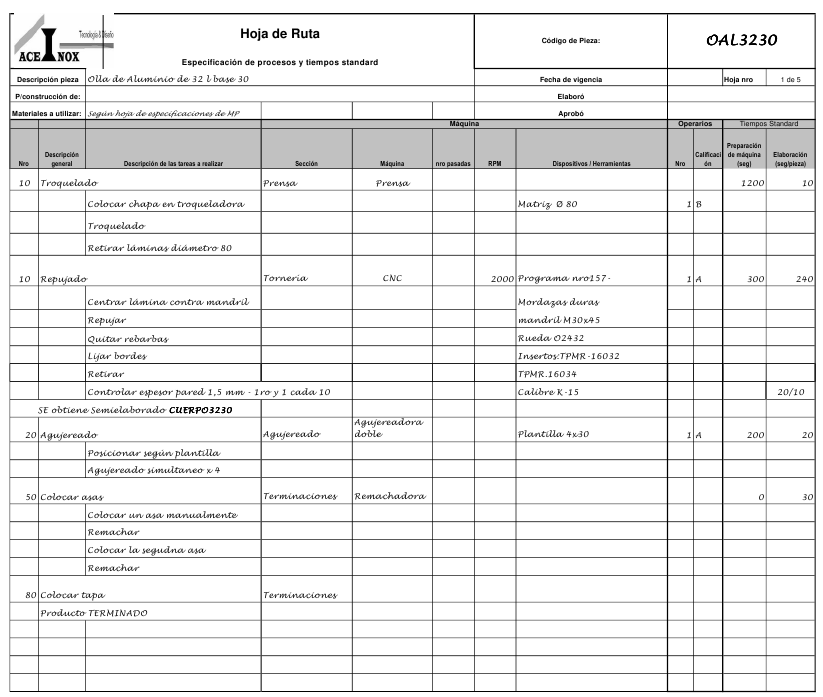
\includegraphics[angle=90,scale=0.95,keepaspectratio=true]{./Circuitos-Teoricos/Produccion/Images/hoja-de-ruta.png}
 % hoja-de-ruta.png: 823x697 pixel, 96dpi, 21.77x18.44 cm, bb=0 0 617 523
\end{center}

\pagebreak
\begin{itemize}
 \item \textbf{Objetivo}: Es un documento en el que se especifican las operaciones que se realizan sobre un mismo artículo hasta el momento de transformarlo en otro.
 \item \textbf{Alcance}: Es un documento interno de la empresa.
\end{itemize}

\subsubsection{Descripción}
\begin{enumerate}
 \item Logo de la empresa.
 \item C\'odigo interno de la pieza.
 \item Fecha de vigencia.
 \item Fecha de elaboraci\'on.
 \item Fecha de aprobaci\'on.
 \item Número de la hoja de ruta.
 \item Descripci\'on de la pieza.
 \item Pedido de construcci\'on.
 \item Materiales a utilizar.
 \item N\'umero de operaci\'on.
 \item Descripci\'on general.
 \item Descripci\'on de las tareas a realizar.
 \item Secci\'on de la m\'aquina. 
 \item Nombre de la m'aquina.
 \item N\'umero de pasadas por la m\'aquina.
 \item N\'umero de revoluciones por minuto para la m\'aquina.
 \item Dispositivos y herramientas.
 \item N\'umero de operario.
 \item Calificaci\'on del operario.
 \item Tiempo standard de preparacion de m\'aquina (segundos).
 \item Tiempo standard de elaboraci\'on (seg/pieza).
\end{enumerate}


\pagebreak
\section{Normas de control interno generales y específicas de Producci\'on}
\begin{itemize}
  \item \textbf{Existencia de inventario permanente o registros contables apropiados:} realización de recuentos físicos periódicos de las existencias, con toma de inventario rotativos, sorpresivos y realizados por personas ajenas a quienes detentan la custodia física de dichos bienes, y de quienes registran los movimientos de los mismos. El inventario físico contribuye a controlar y ajustar los movimientos físicos, evaluar la eficiencia operativa en el manejo de las existencias y sus registraciones, constatar la existencia física y controlar la imputación y valuación contable. Normalmente se debe efectuar un inventario físico total a fin del ejercicio contable.
  \item \textbf{Ajustes de inventario:} Los ajustes por diferencias de inventario deberán estar analizados, justificados y autorizados por un funcionario responsable que sea ajeno a la custodia de los bienes.
  \item \textbf{Custodia de las existencias:} La responsabilidad por la custodia y control de los bienes en existencia, debe recaer sobre una sola persona, a quien se le deben asegurar todas las facilidades de control. El local del depósito debe permitir una protección física adecuada de los bienes.
  Las condiciones del local deben garantizar que no se produzcan deterioros en los productos ( humedad, temperatura, ventilación, etc.)
  \item \textbf{Documentación de todo movimiento de existencias:} Todo movimiento de los bienes en Almacenes, debe estar amparado por el respectivo comprobante, debidamente firmado por un responsable con las atribuciones para realizar los respectivos movimientos.
  \item \textbf{Fijación de puntos de pedido, stocks mínimos y lotes óptimos:} Se recomienda la fijación de stocks de pedido, mínimos, máximos y lotes óptimos de pedido o criterios especiales de reaprovisionamiento.
  \item \textbf{Contratación de seguros adecuados}
\end{itemize}

